% Compile with XeLaTeX

%%%%%%%%%%%%%%%%%%%%%%%
% Option 1: Slides: (comment for handouts)   %
%%%%%%%%%%%%%%%%%%%%%%%
%
%\documentclass[slidestop,compress,mathserif,12pt,t,professionalfonts,xcolor=table]{beamer}
%
%% solution stuff
%\newcommand{\solnMult}[1]{
%\only<1>{#1}
%\only<2->{\red{\textbf{#1}}}
%}
%\newcommand{\soln}[1]{\textit{#1}}

%%%%%%%%%%%%%%%%%%%%%%%%%%%%%%%
% Option 2: Handouts, without solutions (post before class)    %
%%%%%%%%%%%%%%%%%%%%%%%%%%%%%%%

\documentclass[11pt,containsverbatim,handout,xcolor=xelatex,dvipsnames,table]{beamer}

% handout layout
\usepackage{pgfpages}
\pgfpagesuselayout{4 on 1}[letterpaper,landscape,border shrink=5mm]

% solution stuff
\newcommand{\solnMult}[1]{#1}
\newcommand{\soln}[1]{}

% tell pgfpages how to set page sizes in XeLaTeX
\renewcommand\pgfsetupphysicalpagesizes{%
    \pdfpagewidth\pgfphysicalwidth\pdfpageheight\pgfphysicalheight%
}

%%%%%%%%%%%%%%%%%%%%%%%%%%%%%%%%%%%%
% Option 3: Handouts, with solutions (may post after class if need be)    %
%%%%%%%%%%%%%%%%%%%%%%%%%%%%%%%%%%%%

%\documentclass[11pt,containsverbatim,handout,xcolor=xelatex,dvipsnames,table]{beamer}

%% handout layout
%\usepackage{pgfpages}
%\pgfpagesuselayout{4 on 1}[letterpaper,landscape,border shrink=5mm]

%% solution stuff
%\newcommand{\solnMult}[1]{\red{\textbf{#1}}}
%\newcommand{\soln}[1]{\textit{#1}}

%% tell pgfpages how to set page sizes in XeLaTeX
%\renewcommand\pgfsetupphysicalpagesizes{%
%    \pdfpagewidth\pgfphysicalwidth\pdfpageheight\pgfphysicalheight%
%}

%%%%%%%%%%
% Load style file   %
%%%%%%%%%%

%%%%%%%%%%%%%%%%
% Themes
%%%%%%%%%%%%%%%%

% See http://deic.uab.es/~iblanes/beamer_gallery/ for mor options

% Style theme
\usetheme{Pittsburgh}

% Color theme
\usecolortheme{seahorse}

% Font theme
%\usepackage[T1]{fontenc}
%\usepackage[scaled=0.92]{helvet}

%\usepackage[no-math]{fontspec}
%\setsansfont{TeX Gyre Heros}
% "TeX Gyre Heros can be used as a replacement for Helvetica"
% In Unix, unzip the following into ~/.fonts
% In Mac, unzip it, double-click the .otf files, and install using "FontBook"
%   http://www.gust.org.pl/projects/e-foundry/tex-gyre/heros/qhv2.004otf.zip

\usepackage{fontspec}

%%%%%%%%%%%%%%%%
% Packages
%%%%%%%%%%%%%%%%

\usepackage{geometry}
\usepackage{graphicx}
\usepackage{amssymb}
\usepackage{epstopdf}
\usepackage{amsmath}  	% this permits text in eqnarray among other benefits
\usepackage{url}		% produces hyperlinks
\usepackage[english]{babel}
\usepackage[latin1]{inputenc}
\usepackage{colortbl}	% allows for color usage in tables
\usepackage{multirow}	% allows for rows that span multiple rows in tables
\usepackage{color}		% this package has a variety of color options
\usepackage{colortbl}
\usepackage{pgf}
\usepackage{calc}
\usepackage{ulem}
\usepackage{multicol}
\usepackage{textcomp}
\usepackage{txfonts}
\usepackage{listings}
\usepackage{tikz}
\usepackage{fancyvrb}

%%%%%%%%%%%%%%%%
% Remove navigation symbols
%%%%%%%%%%%%%%%%

\beamertemplatenavigationsymbolsempty
\hypersetup{pdfpagemode=UseNone} % don't show bookmarks on initial view

%%%%%%%%%%%%%%%%
% User defined colors
%%%%%%%%%%%%%%%%

% Pantone 2015 Spring colors
% http://iwork3.us/2014/09/16/pantone-2015-spring-fashion-report/
% update each semester or year

\xdefinecolor{custom_blue}{rgb}{0, 0.70, 0.79} % scuba blue
\xdefinecolor{custom_darkBlue}{rgb}{0.11, 0.31, 0.54} % classic blue
\xdefinecolor{custom_orange}{rgb}{0.97, 0.57, 0.34} % tangerine
\xdefinecolor{custom_green}{rgb}{0.49, 0.81, 0.71} % lucite green
\xdefinecolor{custom_red}{rgb}{0.58, 0.32, 0.32} % marsala

\xdefinecolor{custom_lightGray}{rgb}{0.78, 0.80, 0.80} % glacier gray
\xdefinecolor{custom_darkGray}{rgb}{0.54, 0.52, 0.53} % titanium

%%%%%%%%%%%%%%%%
% Template colors
%%%%%%%%%%%%%%%%

\setbeamercolor*{palette primary}{fg=white,bg= custom_blue}
\setbeamercolor*{palette secondary}{fg=black,bg= custom_blue!80!black}
\setbeamercolor*{palette tertiary}{fg=white,bg= custom_blue!80!black!80}
\setbeamercolor*{palette quaternary}{fg=white,bg= custom_blue}

\setbeamercolor{structure}{fg= custom_blue}
\setbeamercolor{frametitle}{bg= custom_blue!90}
\setbeamertemplate{blocks}[shadow=false]
\setbeamersize{text margin left=2em,text margin right=2em}

%%%%%%%%%%%%%%%%
% Styling fonts, bullets, etc.
%%%%%%%%%%%%%%%%

% styling of itemize bullets
\setbeamercolor{item}{fg=custom_blue}
\setbeamertemplate{itemize item}{{{\small$\blacktriangleright$}}}
\setbeamercolor{subitem}{fg=custom_blue}
\setbeamertemplate{itemize subitem}{{\textendash}}
\setbeamerfont{itemize/enumerate subbody}{size=\footnotesize}
\setbeamerfont{itemize/enumerate subitem}{size=\footnotesize}

% styling of enumerate bullets
\setbeamertemplate{enumerate item}{\insertenumlabel.}
\setbeamerfont{enumerate item}{family={\fontspec{Helvetica Neue}}}
\setbeamerfont{enumerate subitem}{family={\fontspec{Helvetica Neue}}}
\setbeamerfont{enumerate subsubitem}{family={\fontspec{Helvetica Neue}}}

% make frame titles small to make room in the slide
\setbeamerfont{frametitle}{size=\small} 

% set Helvetica Neue font for frame and section titles
\setbeamerfont{frametitle}{family={\fontspec{Helvetica Neue}}}
\setbeamerfont{sectiontitle}{family={\fontspec{Helvetica Neue}}}
\setbeamerfont{section in toc}{family={\fontspec{Helvetica Neue}}}
\setbeamerfont{subsection in toc}{family={\fontspec{Helvetica Neue}}}
\setbeamerfont{footline}{family={\fontspec{Helvetica Neue}}}
\setbeamerfont{subsection in toc}{family={\fontspec{Helvetica Neue}}}
\setbeamerfont{block title}{family={\fontspec{Helvetica Neue}}}

%%%%%%%%%%%%%%%%
% Color text commands
%%%%%%%%%%%%%%%%

%orange
\newcommand{\orange}[1]{\textit{\textcolor{custom_orange}{#1}}}

% green
\newcommand{\green}[1]{\textit{\textcolor{custom_green}{#1}}}

% red
\newcommand{\red}[1]{\textit{\textcolor{custom_red}{#1}}}

% dark gray
\newcommand{\darkgray}[1]{\textit{\textcolor{custom_darkGray}{#1}}}

% light gray
\newcommand{\lightgray}[1]{\textit{\textcolor{custom_lightGray}{#1}}}


%%%%%%%%%%%%%%%%
% Custom commands
%%%%%%%%%%%%%%%%

% cancel
\newcommand{\cancel}[1]{%
    \tikz[baseline=(tocancel.base)]{
        \node[inner sep=0pt,outer sep=0pt] (tocancel) {#1};
        \draw[red, line width=0.5mm] (tocancel.south west) -- (tocancel.north east);
    }%
}

% degree
\newcommand{\degree}{\ensuremath{^\circ}}

% cite
\newcommand{\ct}[1]{
\vfill
{\tiny #1}}

% Note
\newcommand{\Note}[1]{
\rule{2.5cm}{0.25pt} \\ \textit{\footnotesize{\textcolor{custom_red}{Note:} \textcolor{custom_darkGray}{#1}}}}

% Remember
\newcommand{\Remember}[1]{\textit{\scriptsize{\textcolor{custom_red}{Remember:} #1}}}

% links: webURL, webLink
\newcommand{\webURL}[1]{\urlstyle{same}{\textit{\textcolor{custom_blue}{\url{#1}}}}}
\newcommand{\webLink}[2]{\href{#1}{\textcolor{custom_blue}{{#2}}}}

% mail
\newcommand{\mail}[1]{\href{mailto:#1}{\textit{\textcolor{custom_blue}{#1}}}}

% highlighting: hl, hlGr, mathhl
\newcommand{\hl}[1]{\textit{\textcolor{custom_blue}{#1}}}
\newcommand{\hlGr}[1]{\textit{\textcolor{custom_green}{#1}}}
\newcommand{\mathhl}[1]{\textcolor{custom_blue}{\ensuremath{#1}}}

% example
\newcommand{\ex}[1]{\textcolor{blue}{{{\small (#1)}}}}

% two col: two columns
\newenvironment{twocol}[4]{
\begin{columns}[c]
\column{#1\textwidth}
#3
\column{#2\textwidth}
#4
\end{columns}
}

% slot (for probability calculations)
\newenvironment{slot}[2]{
\begin{array}{c} 
\underline{#1} \\ 
#2
\end{array}
}

% pr: left and right parentheses
\newcommand{\pr}[1]{
\left( #1 \right)
}

%%%%%%%%%%%%%%%%
% Custom blocks
%%%%%%%%%%%%%%%%

% activity: less commonly used
\newcommand{\activity}[2]{
\setbeamertemplate{itemize item}{{{\small\textcolor{custom_orange}{$\blacktriangleright$}}}}
\setbeamercolor{block title}{fg=white, bg=custom_orange}
\setbeamerfont{block title}{size=\small}
\setbeamercolor{block body}{fg=black, bg=custom_orange!20!white!80}
\setbeamerfont{block body}{size=\small}
\begin{block}{Activity: #1}
#2
\end{block}
}

% app: application exercise
\newcommand{\app}[2]{
\setbeamercolor{block title}{fg=white,bg=custom_green}
\setbeamercolor{block body}{fg=black,bg=custom_green!20!white!80}
\begin{block}{{\small Application exercise: #1}}
#2
\end{block}
}

% disc: discussion question
\newcommand{\disc}[1]{
\setbeamercolor{block body}{bg=custom_blue!25!white!80, fg=custom_blue!55!black!95}
\begin{block}{\vspace*{-3ex}}
#1
\end{block}
}

% clicker: clicker question
\newcommand{\clicker}[1]{
\setbeamercolor{block title}{bg=custom_blue!80!white!50,fg=custom_blue!30!black!90}
\setbeamercolor{block body}{bg=custom_blue!20!white!80,fg=custom_blue!30!black!90}
\begin{block}{\vspace*{-0.2ex}{\footnotesize Clicker question}\vspace*{-0.2ex}}
#1
\end{block}
}

% formula
\newcommand{\formula}[2]{
\setbeamercolor{block title}{bg=custom_blue!40!white!60,fg=custom_blue!55!black!95}
\begin{block}{{\small#1}}
#2
\end{block}
}

% code
\newcommand{\code}[1]{
\newfontfamily{\monaco}{Monaco}
{\monaco {\footnotesize \textcolor{custom_darkBlue}{#1}}}
}

% output
\renewcommand{\output}[1]{
{\monaco {\footnotesize \textcolor{custom_darkGray}{#1}}}
}

%%%%%%%%%%%%%%%%
% Change margin
%%%%%%%%%%%%%%%%

\newenvironment{changemargin}[2]{%
\begin{list}{}{%
\setlength{\topsep}{0pt}%
\setlength{\leftmargin}{#1}%
\setlength{\rightmargin}{#2}%
\setlength{\listparindent}{\parindent}%
\setlength{\itemindent}{\parindent}%
\setlength{\parsep}{\parskip}%
}%
\item}{\end{list}}

%%%%%%%%%%%%%%%%
% Footnote
%%%%%%%%%%%%%%%%

\long\def\symbolfootnote[#1]#2{\begingroup%
\def\thefootnote{\fnsymbol{footnote}}\footnote[#1]{#2}\endgroup}

%%%%%%%%%%%%%%%%
% Graphics
%%%%%%%%%%%%%%%%

\DeclareGraphicsRule{.tif}{png}{.png}{`convert #1 `dirname #1`/`basename #1 .tif`.png}

%%%%%%%%%%%%%%%%
% Slide number
%%%%%%%%%%%%%%%%

\setbeamertemplate{footline}{%
    \raisebox{5pt}{\makebox[\paperwidth]{\hfill\makebox[20pt]{\color{gray}
          \scriptsize\insertframenumber}}}\hspace*{5pt}}

          
%%%%%%%%%%%%%%%%
% Remove page numbers
%%%%%%%%%%%%%%%%

\newcommand{\removepagenumbers}{% 
  \setbeamertemplate{footline}{}
}

%%%%%%%%%%%%%%%%
% TOC slides
%%%%%%%%%%%%%%%%

\AtBeginSection[] 
{ 
  \addtocounter{framenumber}{-1} 
  % 
  {\removepagenumbers 
    \begin{frame}<beamer> 
    \tableofcontents[currentsection] 
  \end{frame} 
  } 
}

%%%%%%%%%%%
% Cover slide info    %
%%%%%%%%%%%

\title{Data Analysis and Statistical Inference}
\subtitle{Introduction}
\author{Sta 101 - Spring 2015}
\date{January 7, 2015}
\institute{Duke University, Department of Statistical Science}


%%%%%%%%%%%%%%%%%%%%%%%%%
% Begin document and set Helvetica Neue font   %
%%%%%%%%%%%%%%%%%%%%%%%%%

\begin{document}
\fontspec[Ligatures=TeX]{Helvetica Neue Light}

%%%%%%%%%%%%%%%%%%%%%%%%%%%%%%%%%%%

% Title Page

\begin{frame}[plain]

\titlepage
\vfill
{\scriptsize \webLink{http://stat.duke.edu/~mc301}{Dr. \c{C}etinkaya-Rundel} \hfill Slides posted at  \webLink{http://bitly.com/sta101sp15}{bitly.com/sta101sp15}}
\addtocounter{framenumber}{-1} 

\end{frame}

%%%%%%%%%%%%%%%%%%%%%%%%%%%%%%%%%%%

\section{General info}

% THIS SECTION CONTAINS COURSE/SYLLABUS INFO
% GO OVER IT QUICKLY AS IT IS LIKELY INFORMATION OVERLOAD
% BUT USEFUL FOR STUDENTS TO HEAR ON THE FIRST DAY
% ESTIMATE - 20 MINUTES

%%%%%%%%%%%%%%%%%%%%%%%%%%%%%%%%%%%

\begin{frame}
\frametitle{Teaching team}

\begin{itemize}

\item Professor: Dr. Mine \c{C}etinkaya-Rundel - \mail{mine@stat.duke.edu}

\item TAs:
\begin{itemize}
\item TBA
\end{itemize}

\end{itemize}

\end{frame}

%%%%%%%%%%%%%%%%%%%%%%%%%%%%%%%%%%%

\begin{frame}
\frametitle{Required materials}

\begin{itemize}

\item OpenIntro Statistics, 2nd Edition

\item i$>$clicker2 - See Google Doc for a list of students selling used clickers (link emailed)

\item (optional) Calculator

\end{itemize}

\end{frame}

%%%%%%%%%%%%%%%%%%%%%%%%%%%%%%%%%%%

\begin{frame}
\frametitle{Webpage}

\vfill

\centering
{\Large 
\webURL{http://bit.ly/sta101sp15}
}

\vfill

\end{frame}

%%%%%%%%%%%%%%%%%%%%%%%%%%%%%%%%%%%

\begin{frame}
\frametitle{Grading}

\begin{center}
\rowcolors{1}{}{custom_lightGray}
\renewcommand\arraystretch{1.25}
{\scriptsize
\begin{tabular}{ r | l }
\textbf{Component} & \textbf{Weight} \\
Attendance \& participation + peer evaluation	& 7.5\% \\
Problem sets							& 10\%  \\ 
Labs									& 10\% \\    
Readiness assessments					& 10\%   \\  
Performance assessments 				& 2.5\%  \\  
Project 1								& 5\%   \\   
Project 2								& 10\% \\   
Midterm 1								& 10\% \\    
Midterm 2 							& 10\% \\    
Final 								& 25\%     
\end{tabular}
}
\end{center}

\begin{itemize}

\item Grades curved at the end of the course after overall averages have been calculated
\begin{itemize}
\item average of 90-100 guaranteed A-
\item average of 80-90 guaranteed B-
\item average of 70-80 guaranteed C-
\end{itemize}

\item The more evidence there is that the class has mastered the material, the more generous the curve will be
\end{itemize}

\end{frame}

%%%%%%%%%%%%%%%%%%%%%%%%%%%%%%%%%%%

\begin{frame}
\frametitle{Course goals and objectives}

{\footnotesize
\begin{itemize}[<alert@+>]
\item Recognize the importance of data collection, identify limitations in data collection methods, and determine how they affect the scope of inference.
\item Use statistical software to summarize data numerically and visually, and to perform data analysis.
\item Have a conceptual understanding of the unified nature of statistical inference.
\item Apply estimation and testing methods to analyze single variables or the relationship between two variables in order to understand natural phenomena and make data-based decisions.
\item Model numerical response variables using a single or multiple explanatory variables.
\item Interpret results correctly, effectively, and in context without relying on statistical jargon.
\item Critique data-based claims and evaluate data-based decisions.
\item Complete two research projects: one that focuses on statistical inference and one that focuses on modeling. 
\end{itemize}
}

\end{frame}

%%%%%%%%%%%%%%%%%%%%%%%%%%%%%%%%%%%

\begin{frame}
\frametitle{Learning units and course outline}

{\footnotesize
\begin{itemize}[<+->]
\item \hl{Unit 1 - Intro to data:} Observational studies and non-causal inference, principles of experimental design and causal inference, exploratory data analysis, and introduction to simulation-based statistical inference
\item \hl{Unit 2 - Probability \& distributions:} Basics of probability and chance processes, Bayesian perspective in statistical inference, the normal and binomial distributions
\item \hl{Unit 3 - Framework for inference:} CLT, sampling distributions, and introduction to theoretical inference
\begin{itemize}
\item Midterm 1
\end{itemize}
\item \hl{Unit 4 - Statistical inference for numerical variables}
\item \hl{Unit 5 - Statistical inference for categorical variables}
\begin{itemize}
\item Project 1 \& Midterm 2
\end{itemize}
\item \hl{Unit 6 - Simple linear regression:} Bivariate correlation and causality, introduction to modeling
\item \hl{Unit 7 - Multiple linear regression:} More advanced modeling with multiple predictors
\begin{itemize}
\item Project 2 \& Final
\end{itemize}
\end{itemize}
}

\end{frame}

%%%%%%%%%%%%%%%%%%%%%%%%%%%%%%%%%%%

\begin{frame}
\frametitle{Course structure}

\begin{itemize}[<alert@+>]
\item Set of learning objectives and required and suggested readings, videos, etc. for each unit
\item Prior to beginning the unit, watch the videos and/or complete the readings and familiarize yourselves with the learning objectives
\item Begin a new unit with a readiness assessment: individual, then team 
\item Class time: split between lecture, discussion/application, and lab
\item Complement your learning with problem sets
\item Wrap up a unit with a performance assessment
\end{itemize}

\end{frame}

%%%%%%%%%%%%%%%%%%%%%%%%%%%%%%%%%%%

\begin{frame}
\frametitle{Teams}

\begin{itemize}
\item Highly functional teams of learners based on survey and pre-test

\item Team members first point of contact

\item Application exercises, labs, team readiness assessments, projects

\item Study together, but anything that is not explicitly a team assignment must be your own work

\item Peer evaluations to ensure that all team members contribute to the success of the group and to address any potential issues early on
\begin{itemize}
\item If you feel that there are issues within your team, you are encouraged to discuss it with your team members and to bring it to my or your TA's attention ASAP (don't wait till things get worse)
\end{itemize}

\end{itemize}

\end{frame}

%%%%%%%%%%%%%%%%%%%%%%%%%%%%%%%%%%%

\begin{frame}
\frametitle{Clickers}

\red{Objective:} Two-way communication and instant feedback

\begin{itemize}
\item Readiness assessments (graded for accuracy)

\item Questions throughout lecture (graded for participation)
\begin{itemize}
\item to get credit for the day you must respond to at least 75\% of the questions
\item up to three unexcused late arrivals or absences will not affect your clicker grade
\end{itemize}

\item Register your clicker
\begin{itemize}
\item \webURL{https://www1.iclicker.com/register-clicker} (Student ID = Net ID)
\item grading starts Mon, Jan 26
\end{itemize}

\end{itemize}

\end{frame}

%%%%%%%%%%%%%%%%%%%%%%%%%%%%%%%%%%%

\begin{frame}
\frametitle{Attendance \& participation}

\red{Objective:} Make you an active participant and help me pace the class 

\begin{itemize}

\item Attendance and participation during class, as well as your activity on Piazza make up a non-insignificant portion of your grade in this class

\item Might sometimes call on you during the class discussion, however it is your responsibility to be an active participant without being called on

\end{itemize}

\end{frame}

%%%%%%%%%%%%%%%%%%%%%%%%%%%%%%%%%%%

\begin{frame}
\frametitle{Problem sets (PS)}

\red{Objective:} Help you develop a more in-depth understanding of the material and help you prepare for exams and projects

\begin{itemize}

\item Questions from the textbook

\item Show \emph{all} your work to receive credit

\item \hl{Required format:} Use one of the following, no other submission types will be accepted
\begin{itemize}
\item Type your answers in the text box on Sakai and attach any plots/images as separate files, properly named
\item Attach a PDF (\emph{not} Word, Google Doc, etc.) of your answers
\end{itemize}

\item Welcomed and encouraged to work with others, but turn in your own work

\item No make-ups, excused absences (e.g. STINF) do not excuse homework

\item Lowest PS score will be dropped

\end{itemize}

\end{frame}

%%%%%%%%%%%%%%%%%%%%%%%%%%%%%%%%%%%

\begin{frame}[fragile]
\frametitle{Labs}

\red{Objective:} Give you hands on experience with data analysis using statistical software and provide you with tools for the projects

\begin{itemize}

\item Work in teams: author / discussants

\item Must be present in lab session to get credit

\item Lowest lab score will be dropped

\end{itemize}

\vfill

\pause

\activity{Get started with R/RStudio}{
\begin{itemize}
    \setlength{\itemsep}{0pt}
    \setlength{\parskip}{0pt}
\item Go to the course website, \webURL{http://bit.ly/sta101sp15}, and click on the RStudio link on the top right
\item Log in using your Net ID and password
\item In the Console, generate a random number between 1 and 5, and introduce yourself to that many people sitting around you:
\Rcode{sample(1:5, size = 1)}
\end{itemize}
}

\end{frame}

%%%%%%%%%%%%%%%%%%%%%%%%%%%%%%%%%%%

\begin{frame}
\frametitle{Readiness assessments (RA)}

\red{Objective:} Encourage you to watch the videos and/or complete the reading assignment and review the learning objectives prior to coming to class as well as evaluate your conceptual understanding of the unit's material

\begin{itemize}

\item 10 multiple choice questions, at the beginning of a unit

\item Conceptual questions addressing the learning objectives of the new unit, assessing familiarity and reasoning, not mastery

\item Take the individual RA using clickers, then re-take in teams

\item Individual RA score 3/4 of grade, team RA score 1/4 \& your input during the team portion will factor into your participation grade

\item Lowest RA score will be dropped

\end{itemize}

\end{frame}

%%%%%%%%%%%%%%%%%%%%%%%%%%%%%%%%%%%

\begin{frame}
\frametitle{Performance assessments (PA)}

\red{Objective:} Evaluate your mastery of the material by the end of a unit and give you instant feedback on your performance.

\begin{itemize}

\item 10 multiple choice questions, at the end of a unit

\item Taken individually on Sakai

\item Lowest PA score will be dropped

\end{itemize}

\end{frame}

%%%%%%%%%%%%%%%%%%%%%%%%%%%%%%%%%%%

\begin{frame}
\frametitle{Projects}

\red{Objective:} Give you independent applied research experience using real data and statistical methods

\begin{itemize}

\item Project 1: For a parameter of interest to you, you will describe the relevant data, compute a confidence interval and conduct a hypothesis test, and summarize your findings in a written, fully reproducible, data analysis report

\item Project 2: Use all (relevant) techniques learned in this class to analyze a dataset provided by me, and share your results in a poster session

\item Must complete both projects and score at least 30\% of the points on each project in order to pass this class

\end{itemize}

\end{frame}

%%%%%%%%%%%%%%%%%%%%%%%%%%%%%%%%%%%

\begin{frame}
\frametitle{Exams}

\begin{center}
\rowcolors{1}{}{custom_lightGray}
\renewcommand\arraystretch{1.25}
{\footnotesize
\begin{tabular}{ r | l }
Midterm 1								& Wed, Feb 18 \\    
Midterm 2 							& Wed, Mar 25 \\    
Final 								& Sat, May 2 (2-5pm)     
\end{tabular}
}
\end{center}

\begin{itemize}

\item Exam dates cannot be changed, no make-up exams will be given

\item If you cannot take the exams on these dates you should drop this class

\item Calculator + cheat sheet allowed

\end{itemize}

\end{frame}

%%%%%%%%%%%%%%%%%%%%%%%%%%%%%%%%%%%

\begin{frame}
\frametitle{Email \& Piazza}

\begin{itemize}

\item I will regularly send announcements by email, so make sure to check your email  daily

\item Any \emph{non-personal} questions related to the material covered in class, problem sets, labs, projects, etc. should be posted on Piazza forum

\item Before posting a new question please make sure to check if your question has already been answered, and answer others' questions

\item Use informative titles for your posts

\item It is more efficient to answer most statistical questions ``in person" so make use of OH

\end{itemize}

\end{frame}

%%%%%%%%%%%%%%%%%%%%%%%%%%%%%%%%%%%

\begin{frame}
\frametitle{Students with disabilities}

Students with disabilities who believe they may need accommodations in this class are encouraged to contact the \webLink{http://www.access.duke.edu/students/requesting/index.php}{Student Disability Access Office} at (919) 668-1267 as soon as possible to better ensure that such accommodations can be made

\vfill

\ct{\webURL{http://www.access.duke.edu/students/requesting/index.php}}

\end{frame}

%%%%%%%%%%%%%%%%%%%%%%%%%%%%%%%%%%%

\begin{frame}
\frametitle{Late work policy}

\begin{itemize}

\item Late work policy for problem sets and labs reports:
\begin{itemize}
\item next day: lose 30\% of points (within 24 hours of due date)
\item later than next day: lose all points
\end{itemize}

\item Late work policy for projects: 10\% off for each day late

\end{itemize}

\end{frame}

%%%%%%%%%%%%%%%%%%%%%%%%%%%%%%%%%%%

\begin{frame}
\frametitle{Regrade policy}

Regrade requests must be made \hl{within 3 days} of when the assignment is returned, and must be submitted in writing 

\begin{itemize}

\item These will be honored if points were tallied incorrectly, or if you feel your answer is correct but it was marked wrong

\item No regrade will be made to alter the number of points deducted for a mistake

\item There will be no grade changes after the final exam

\end{itemize}

\end{frame}

%%%%%%%%%%%%%%%%%%%%%%%%%%%%%%%%%%%

\begin{frame}
\frametitle{Make up policy}

\begin{itemize}

\item No make-up for attendance, individual and team readiness assessments, labs, problem sets, projects, or exams

\item If the midterm exam must be missed due to a documented medical excuse, absence must be officially excused \hl{in advance}, in which case the missing exam score will be imputed using the final exam score

\item The final exam must be taken at the stated time

\item You must take the final exam and turn in the projects in order to pass this course

\end{itemize}

\end{frame}

%%%%%%%%%%%%%%%%%%%%%%%%%%%%%%%%%%%

\begin{frame}
\frametitle{Other policies}

\begin{itemize}

\item Clickers may not be shared, and the clicker registered to a person may only be used by that person, failure to abide by this will result in a 0 clicker grade for everyone involved

\item Use of disallowed materials (textbook, class notes, web references, any form of communication with classmates or other persons, etc.) during exams will not be tolerated

\end{itemize}

\end{frame}

%%%%%%%%%%%%%%%%%%%%%%%%%%%%%%%%%%%%

\begin{frame}
\frametitle{Academic Dishonesty}

Any form of academic dishonesty will result in an immediate 0 on the given assignment and will be reported to the Office of Student Conduct. Additional penalties may also be assessed if deemed appropriate. If you have any questions about whether something is or is not allowed, ask me beforehand.

Some examples:

\begin{itemize}

\item Use of disallowed materials (including any form of communication with classmates or accessing the web) during exams and readiness assessments

\item Plagiarism of any kind

\item Use of outside answer keys or solution manuals for the homework

\end{itemize}

\end{frame}

%%%%%%%%%%%%%%%%%%%%%%%%%%%%%%%%%%%%

\begin{frame}
\frametitle{Tips for success}

{\footnotesize
\begin{itemize}[<alert@+>]
\item Complete the reading before a new unit begins, and then review again after the unit is over.
\item Be an active participant during lectures and labs.
\item Ask questions - during class or office hours, or by email. Ask me, your TAs, and your classmates.
\item Do the problem sets - start early and make sure you attempt and understand all questions.
\item Start your projects early and and allow adequate time to complete them.
\item Give yourself plenty of time time to prepare a good cheat sheet for exams. This requires going through the material and taking the time to review the concepts that you're not comfortable with.
\item Do not procrastinate - don't let a unit go by with unanswered questions as it will just make the following unit's material even more difficult to follow. 
\end{itemize}
}

\end{frame}

%%%%%%%%%%%%%%%%%%%%%%%%%%%%%%%%%%%%

\begin{frame}
\frametitle{To do}

\begin{itemize}

\item Download or purchase the textbook

\item Obtain and register your clicker
\begin{itemize}
\item \webURL{https://www1.iclicker.com/register-clicker} (Student ID = Net ID)
\end{itemize}

\item Complete the pretest and survey

\item Read the syllabus and let me know if you have any questions

\item Take the performance assessment (PA 0) by Friday, Jan 9, 11:59pm (on course policies etc., not graded, for practice with the quiz module on Sakai)

\item Start reviewing the resources for Unit 1 - readiness assessment on Monday (not graded, for practice)

\end{itemize}

\end{frame}

%%%%%%%%%%%%%%%%%%%%%%%%%%%%%%%%%%%%

\section{Example: Baby names}

%%%%%%%%%%%%%%%%%%%%%%%%%%%%%%%%%%%%

\begin{frame}
\frametitle{Baby names in the US}

\begin{itemize}

\item Each year the Social Security Administration collects and releases data on the how many babies are given a certain name

\item They released these data for years 1880 onwards for each gender

\item For privacy reasons they restrict the list of names to those with at least 5 occurrences

\end{itemize}

\end{frame}

%%%%%%%%%%%%%%%%%%%%%%%%%%%%%%%%%%%%

\begin{frame}
\frametitle{Top 10 baby names for 2013}

\begin{center}
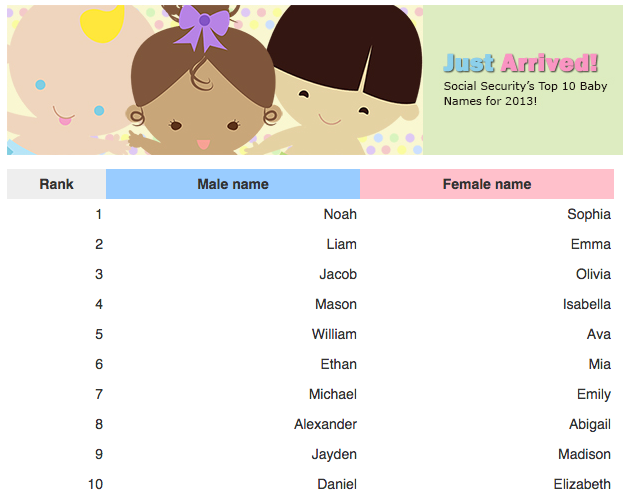
\includegraphics[width=0.8\textwidth]{figures/babynames2013}
\end{center}

\ct{\webURL{http://www.ssa.gov/oact/babynames}}

\end{frame}

%%%%%%%%%%%%%%%%%%%%%%%%%%%%%%%%%%%%

\begin{frame}
\frametitle{Name voyager}

\begin{center}
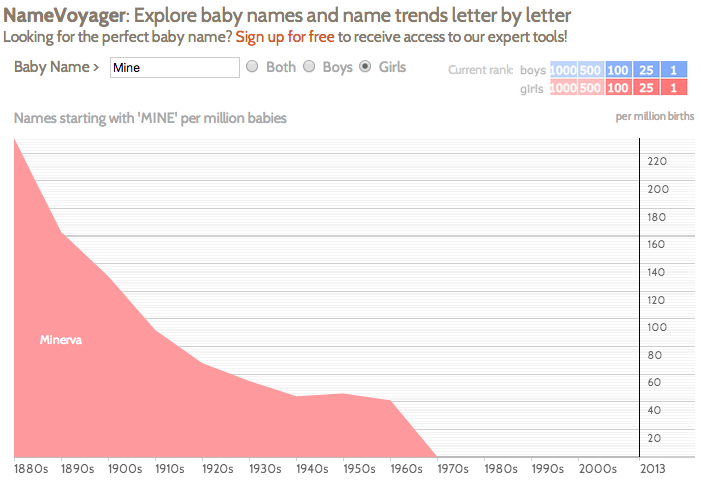
\includegraphics[width=0.8\textwidth]{figures/namevoyager_mine}
\end{center}

\ct{\webURL{http://www.babynamewizard.com/voyager}}

\end{frame}

%%%%%%%%%%%%%%%%%%%%%%%%%%%%%%%%%%%%

\begin{frame}
\frametitle{Names and ages}

\begin{center}
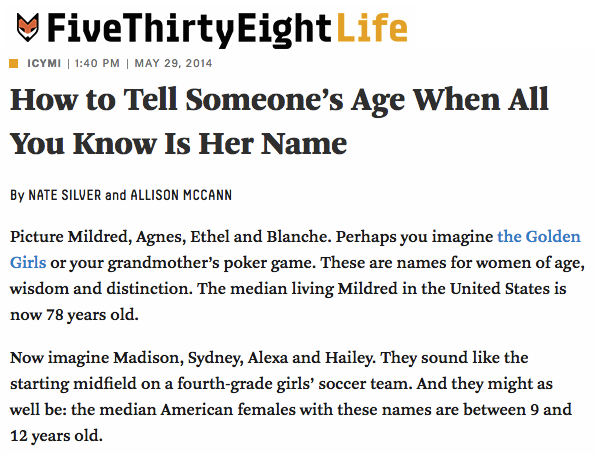
\includegraphics[width=0.8\textwidth]{figures/nameage538}
\end{center}

\ct{\webURL{http://fivethirtyeight.com/features/how-to-tell-someones-age-when-all-you-know-is-her-name}}

\end{frame}

%%%%%%%%%%%%%%%%%%%%%%%%%%%%%%%%%%%%

% THE FOLLOWING 4 SLIDES CONTAIN IMAGES EDITED FOR THIS COURSE
% EITHER UPDATE IMAGES WITH NAME COUNTS FROM YOUR COURSE
% OR OMIT THESE IMAGES AND JUST DISCUSS THE ARTICLE GENERALLY

\begin{frame}
\frametitle{}

\vspace{-0.45cm}

\begin{center}
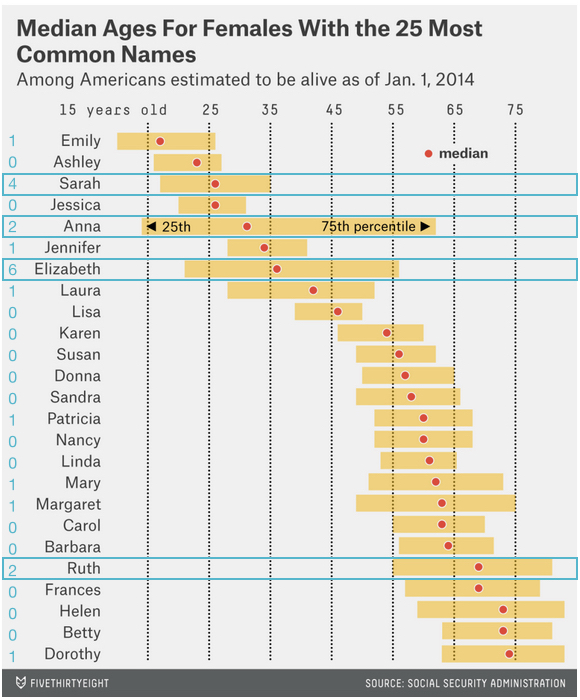
\includegraphics[width=0.7\textwidth]{figures/popnamesclass538_female}
\end{center}

\end{frame}

%%%%%%%%%%%%%%%%%%%%%%%%%%%%%%%%%%%%

\begin{frame}
\frametitle{}

\vspace{-0.45cm}

\begin{center}
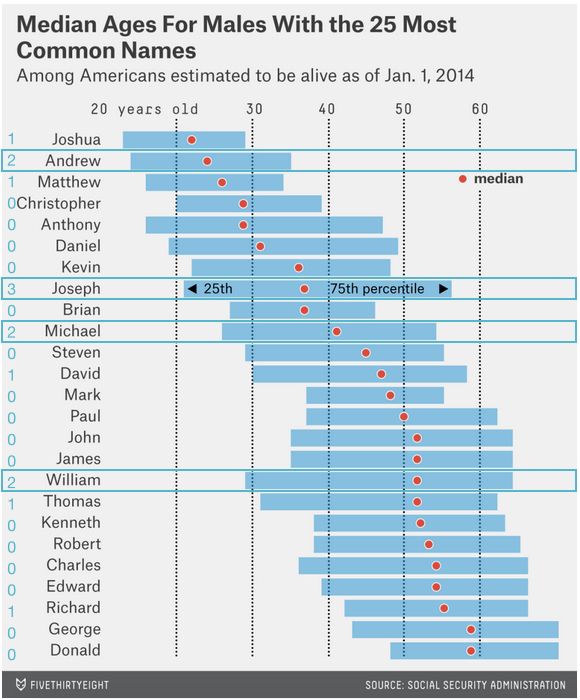
\includegraphics[width=0.7\textwidth]{figures/popnamesclass538_male}
\end{center}

\end{frame}

%%%%%%%%%%%%%%%%%%%%%%%%%%%%%%%%%%%%

\begin{frame}
\frametitle{}

\begin{center}
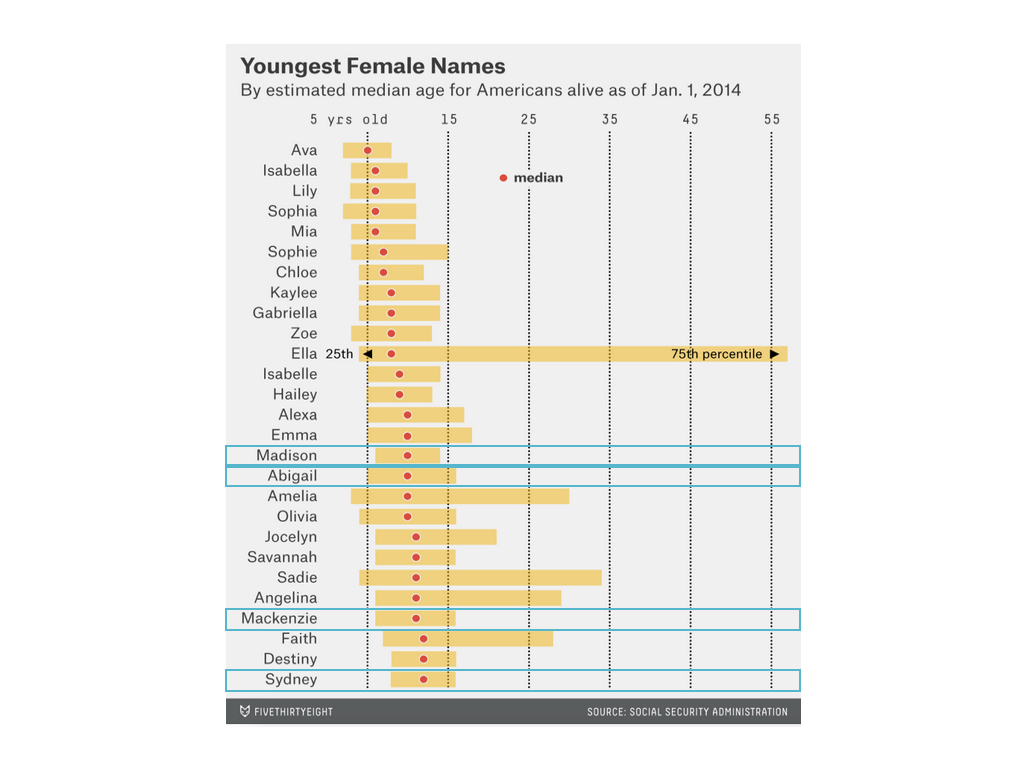
\includegraphics[width=\textwidth]{figures/youngnamesclass538_female}
\end{center}

\end{frame}

%%%%%%%%%%%%%%%%%%%%%%%%%%%%%%%%%%%%

\begin{frame}
\frametitle{}

\begin{center}
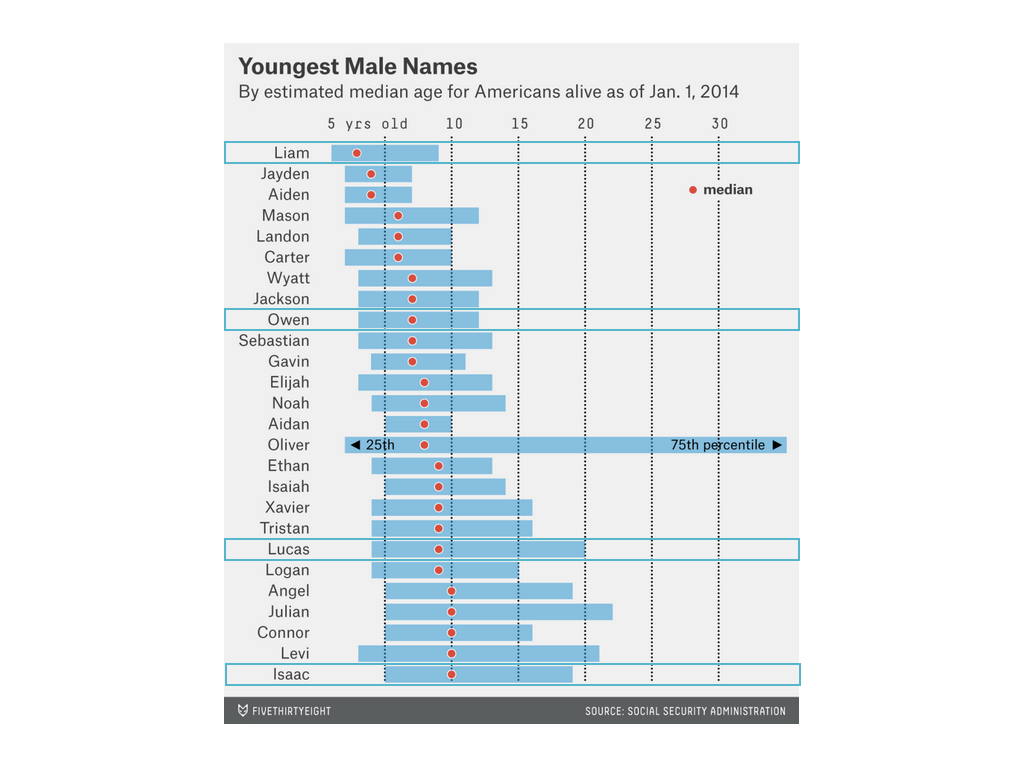
\includegraphics[width=\textwidth]{figures/youngnamesclass538_male}
\end{center}

\end{frame}

%%%%%%%%%%%%%%%%%%%%%%%%%%%%%%%%%%%%

\section{Example: Geotagged data}

%%%%%%%%%%%%%%%%%%%%%%%%%%%%%%%%%%%%

\begin{frame}
\frametitle{}

\clicker{Do you geotag your posts on social networking sites, like Facebook, 
Twitter, Instagram, etc.?}

\begin{enumerate}[(a)]
\item yes
\item no
\end{enumerate}

\end{frame}

%%%%%%%%%%%%%%%%%%%%%%%%%%%%%%%%%%%%

\begin{frame}
\frametitle{Maps based on clicker tags}

\twocol{0.65}{0.35}
{
\begin{center}
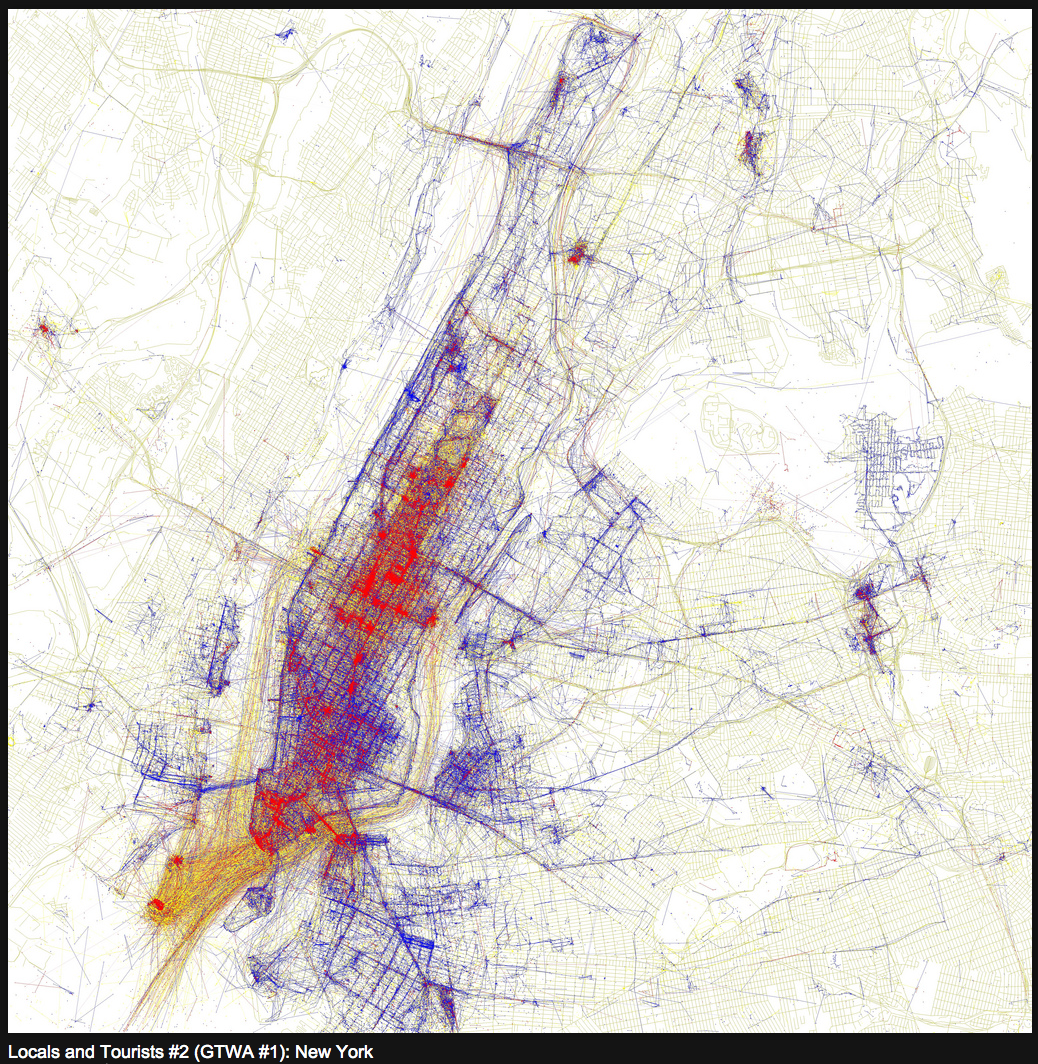
\includegraphics[width=\textwidth]{figures/flickr_ny}
\end{center}
}
{
\begin{itemize}
\item[] \textcolor{red}{tourists}
\item[] \textcolor{blue}{local}
\item[] \textcolor{yellow}{both}
\end{itemize}
}

\ct{\webURL{http://aaronstraupcope.com}}

\end{frame}

%%%%%%%%%%%%%%%%%%%%%%%%%%%%%%%%%%%%

\section{Why study statistics?}

%%%%%%%%%%%%%%%%%%%%%%%%%%%%%%%%%%%%

\begin{frame}
\frametitle{Why study statistics?}

\begin{center}

\includegraphics[width=0.55\textwidth]{figures/lottery}
\end{center}

\end{frame}

%%%%%%%%%%%%%%%%%%%%%%%%%%%%%%%%%%%%

\begin{frame}
\frametitle{Why study statistics?}

\begin{center}
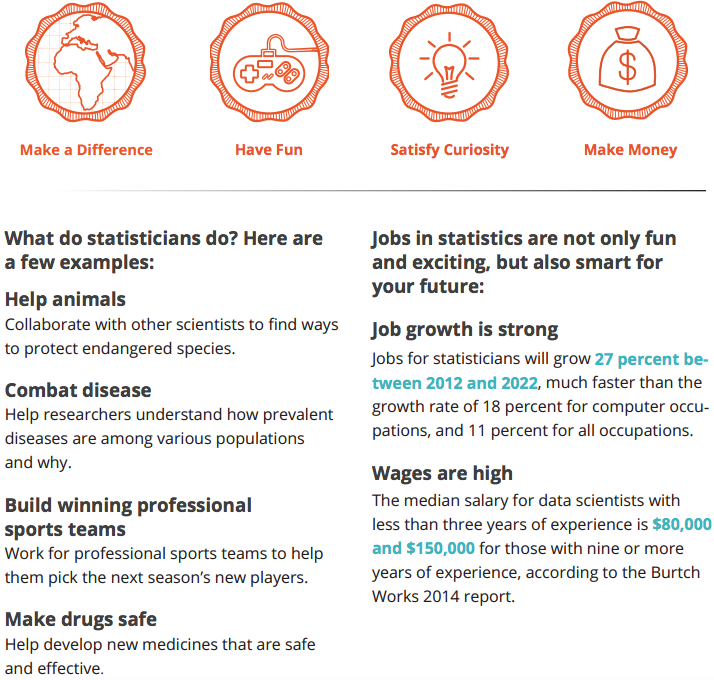
\includegraphics[width=0.7\textwidth]{figures/why_stats}
\end{center}

\vspace{-0.25cm}

\ct{\webURL{http://thisisstatistics.org}}

\end{frame}

%%%%%%%%%%%%%%%%%%%%%%%%%%%%%%%%%%%%

\section{Class survey [time permitting]}

%%%%%%%%%%%%%%%%%%%%%%%%%%%%%%%%%%%%

\begin{frame}
\frametitle{}

\activity{Class survey}
{
\begin{itemize}
    \setlength{\itemsep}{0pt}
    \setlength{\parskip}{0pt}
\item One of your first tasks in this class is to help design a survey. This survey will be completed \emph{anonymously}. It will (ideally) have information on \emph{variables you are interested in}. When writing your question consider whether you would feel comfortable answering it on an anonymous survey.

\item Work with 3-4 classmates to come up with a survey question, and add it to Google Doc linked below. Make sure that the wording of the question is clear, and (if categorical) the answer choices make sense.
\begin{center}
\webURL{http://bit.ly/sta101sp15_ClassSurvey}
\end{center}

\item Before adding a question check to make sure that it hasn't already been added. If your question is already there, but you can suggest a clearer / better wording, add it as ``alternative wording" underneath the original question.
\end{itemize}
}

\end{frame}

%%%%%%%%%%%%%%%%%%%%%%%%%%%%%%%%%%%%

\end{document}